\section{Transceiver}
In the past the number of components was important for transceivers, whereas today it's chip area. Since it is not possible to build a very shallow bandpass filter with only a few components, different transceivers were developed in the past. 
\subsection{Heterodyne Receiver and Image Rejection}
One of them was the superheterodyne receiver, which multiplies the receiving signal with a local oscillator signal as it can be seen in \autoref{fig:typical_superheterodyne_receiver}. Thereby, the lower resulting frequency is often called intermediate frequency ($\omega_{IF}$ or $f_{IF}$).

The bandpass at the beginning of \autoref{fig:typical_superheterodyne_receiver} is used to suppress out-of-band signals. Furthermore, an amplifier is present which might cause issues when the signal is to strong since the amplifier is then not working in its linear region any more. The amplifier is needed because of the mixer, since the mixer has an insertion loss. The IF bandpass filter is used filter out unwanted frequencies and to select the correct channel. To change the receiving frequency one has to changes the oscillator frequency, since the second bandpass is normally constant.\newline
So the RF bandpass is used to do the band selection and remove the image frequency and the if bandpass selects the channel. Sometimes there are two RF filters (one before and one after the amplifier) this is done to keep the insertion loss quite low. $\Rightarrow$ first filter is not very good, but has nearly no insertion loss second filter has more insertion loss, but signal was already amplified.\newline
The different symbols mean the following:
\begin{itemize}
    \item $\omega_{IF}$ = intermediate frequency (difference between $\omega_{LO}$ and $\omega_{RF}$)
    \item $\omega_{LO}$ = local oscillator
    \item $\omega_{RF}$ = radio frequency signal
\end{itemize}
\begin{figure}[ht]
  \centering
  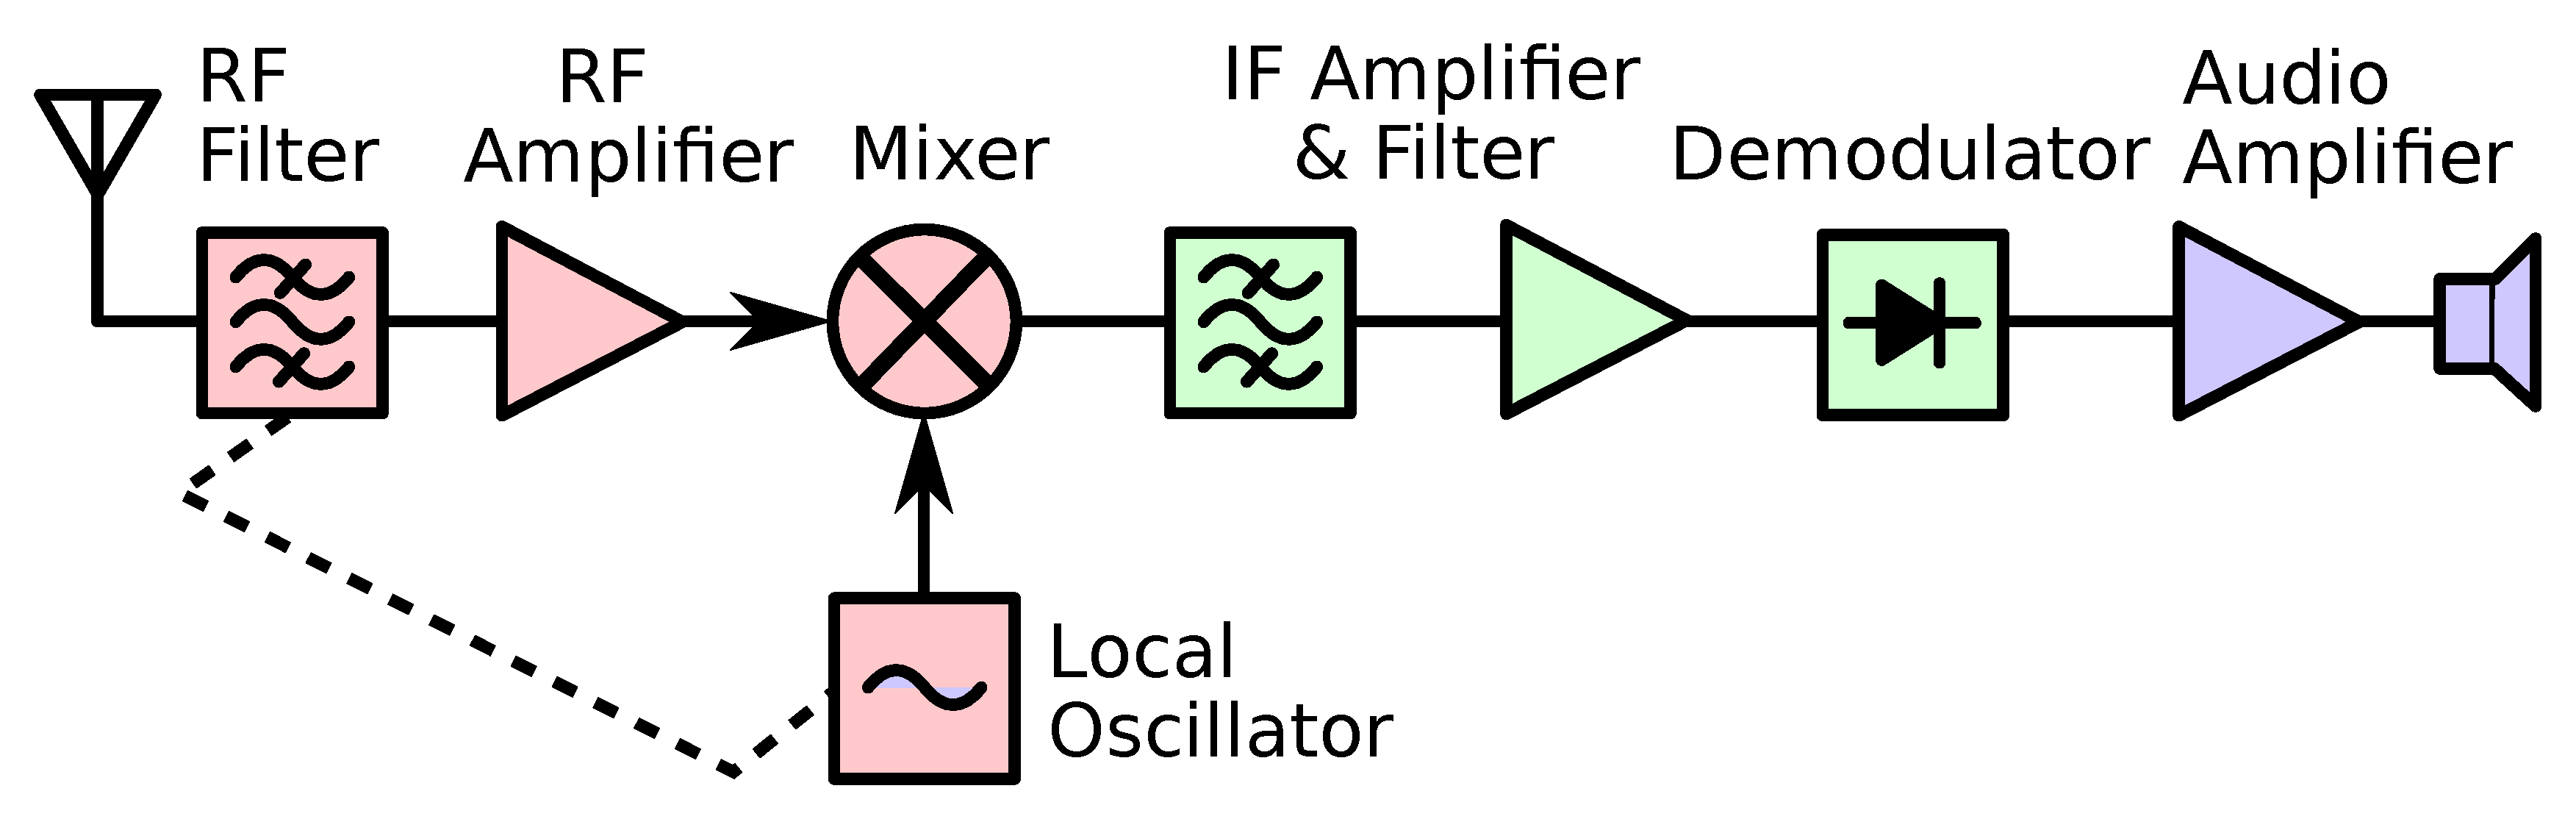
\includegraphics[width=8cm]{images/Superheterodyne1.pdf}
  \caption{typical superheterodyne receiver}
  \label{fig:typical_superheterodyne_receiver}
\end{figure}
\subsubsection{Mixing Processes}\mbox{}\\
To design a superheterodyne receiver, one must be familiar with the trigonometric identities especially with the product identities, which can be seen in \autoref{eq:trigonometric_product_identity}. From those one can then derive \autoref{eq:mixer_output}.
\begin{equation}\label{eq:trigonometric_product_identity}
\begin{aligned}
\sin \alpha \cos \beta &=\frac{\sin (\alpha+\beta)+\sin (\alpha-\beta)}{2} \\
\cos \alpha \cos \beta &=\frac{\cos (\alpha+\beta)+\cos (\alpha-\beta)}{2} \\
\sin \alpha \sin \beta &=\frac{\cos (\alpha-\beta)-\cos (\alpha+\beta)}{2}
\end{aligned}
\end{equation}
\begin{equation}\label{eq:mixer_output}
f_{I F}=\left|f_{R F} \pm f_{L O}\right|
\end{equation}
Due to the properties derived in the formulas above, one could think it's super easy to to get a RF signal to a lower one. The only issue one has is that the received signal is not ideal, one has always some noise on it and one can not create ideal bandpass filters. Which means when $\omega_{LO}$ is chosen to small and the bandpass is to large the new signal on the frequency $\omega_{LO}$ is overlapped by the image frequency (frequency which is mapped to the same $f_{IF}$ as the $f_{RF}$ signal). \newline For example in \autoref{fig:image_freq_1} when we choose $f_{LO}$ to be $f_{LO_1}$ the $f_{RF}$ and $f_{IM_1}$ produce the frequency $f_{IF}$ according to \autoref{eq:mixer_output}. Due to that, one needs a bandpass filter as it can be seen in \autoref{fig:image_freq_2}. There the bandpass filter is not ideal and still some noise from $f_{IM_1}$ superimposes the signal on $f_{IF}$. In \autoref{fig:image_freq_1} and \autoref{fig:image_freq_2} one also sees the smaller $\omega_{IF}$ gets the better the bandpass must be. Furthermore one sees that the image frequency is given by \autoref{eq:image_frequency}.
\begin{equation}\label{eq:image_frequency}
f_{I M}=f_{R F} \pm 2 f_{I F}
\end{equation}
\begin{figure}[ht]
  \centering
  \resizebox{1\textwidth}{!}{\subimport{images/}{spectrum_3.tex}}
  \caption{Image frequencies without bandpass}
  \label{fig:image_freq_1}
\end{figure}
\begin{figure}[ht]
  \centering
  \resizebox{1\textwidth}{!}{\subimport{images/}{spectrum_4.tex}}
  \caption{Image frequencies with bandpass}
  \label{fig:image_freq_2}
\end{figure}


\subsubsection{Zero-if conversion}
A direct-conversion receiver (DCR), also known as homodyne, synchrodyne, or zero-IF receiver, is a radio receiver design that demodulates the incoming radio signal using synchronous detection driven by a local oscillator whose frequency is identical to, or very close to the carrier frequency of the intended signal. The benefit is that one does not have image frequencies and no need of huge analogue filters is needed. The drawback is the receiver topology is more complicated. One needs to do a hilbert transform. Exactly 90 degree phase shift is required.\newline Direct multiplying the RF input signal is only possible when \autoref{eq:direct_conversion} is fullfilled.
\begin{equation}\label{eq:direct_conversion}
\underline{S}\left(f_c-\Delta f\right)=\underline{S}^*\left(f_c+\Delta f\right)
\end{equation}

For example one has the signal $(\sin (x \times 2)+\sin (x \times 2.1)-\sin (x \times 1.9))$ and want to transform it with this mehtod, therefore one multiplies it with $\sin (2 x)$ which results in the following:  $\sin (2 x)(\sin (x \times 2)+\sin (x \times 2.1)-\sin (x \times 1.9))$ which results in the following: $\frac{1}{2}(-\cos (4.1 x)-\cos (4 x)+\cos (3.9 x)+1)$ from which one can see  that some part of the signal is missing in the baseband. But when also doing the multiplication with a 90 degree pahse shifted signal one also gets this part as it can be seen in the following: $\cos (2 x)(\sin (x \times 2)+\sin (x \times 2.1)-\sin (x \times 1.9))$ which is $\frac{1}{2}(\sin (4.1 x)+\sin (4 x)-\sin (3.9 x)+2 \sin (0.1 x))$
$$
\begin{aligned}
    &\cos (2\cdot \omega)(\sin (2\cdot \omega)+\sin (2.1\cdot \omega)-\sin (1.9\cdot \omega))&=\frac{1}{2}(\sin (4.1\cdot \omega)+\sin (4\cdot \omega)-\sin (3.9\cdot \omega)+2 \sin (0.1\cdot \omega))\\
    &\cos (2\cdot \omega)(\sin (2\cdot \omega)-\sin (2.1\cdot \omega)+\sin (1.9\cdot \omega))&=\frac{1}{2}(\sin (4.1\cdot \omega)+\sin (4\cdot \omega)-\sin (3.9\cdot \omega)-2 \sin (0.1\cdot \omega))\\
\end{aligned}
$$
$$
\begin{aligned}
    &e^{-2 i \omega}(\sin (1.9 \omega)+\sin (2 \omega)-\sin (2.1 \omega)) =\frac{1}{2} i e^{-4 i \omega}-\frac{1}{2} i e^{(-0.1 i) \omega}+\frac{1}{2} i e^{(0.1 i) \omega}+\frac{1}{2} i e^{(-3.9 i) \omega}-\frac{1}{2} i e^{(-4.1 i) \omega}+-\frac{i}{2}\\
    &=\frac{1}{2} i(2 i \sin (0.1 \omega)-i \sin (3.9 \omega)-i \sin (4 \omega)+ i \sin (4.1 \omega)+\cos (3.9 \omega)+\cos (4 \omega)-\cos (4.1 \omega)-1)\\
\end{aligned}
$$

\paragraph{Broadband phase shifting}
\begin{enumerate}
    \item Show that a broadband 90$^{\circ}$ phase shifting can be realized using the circuit topology in \autoref{fig:phase_shifter}
    $$
    \underline{T_1}=\frac{U_2}{\underline{U}_1}=\frac{1}{1+j \omega R C}
    $$
    $$
    \underline{T_2}=\frac{\underline{U}_2^{\prime}}{\underline{U_1^{\prime}}}=\frac{j \omega R C}{1+j \omega R C}
    $$
    $$
    \varphi=\arg \left\{\underline{I}_2\right\}-\arg \left\{\underline{T}_1\right\}=90^{\circ}-\arctan \{\omega R C\}-(-\arctan \{\omega R C\})=90^{\circ}, \forall \omega
    $$
    \item What would be the amplitude characteristics without limiting amplifiers?
    $$
    \left|\frac{T_2}{T_1}\right|=\omega R C
    $$
    $$
    \Rightarrow \text { with increasing frequency, the amplitude of } V_{\text {out2 }} \text { increases with respect to } V_{\text {out1 }}
    $$
\paragraph{90$^{\circ}$ phase shifter}
Find an almost ideal 90$^{\circ}$ phase shifter topology consisting of a 'divide by 2' counter and an
oscillator.\newline
\begin{itemize}
    \item Operate the oscillator on twice the output signal frequency
    \item Use a 'divide by two' counter
\end{itemize}
\end{enumerate}
\begin{figure}[ht]
  \centering
  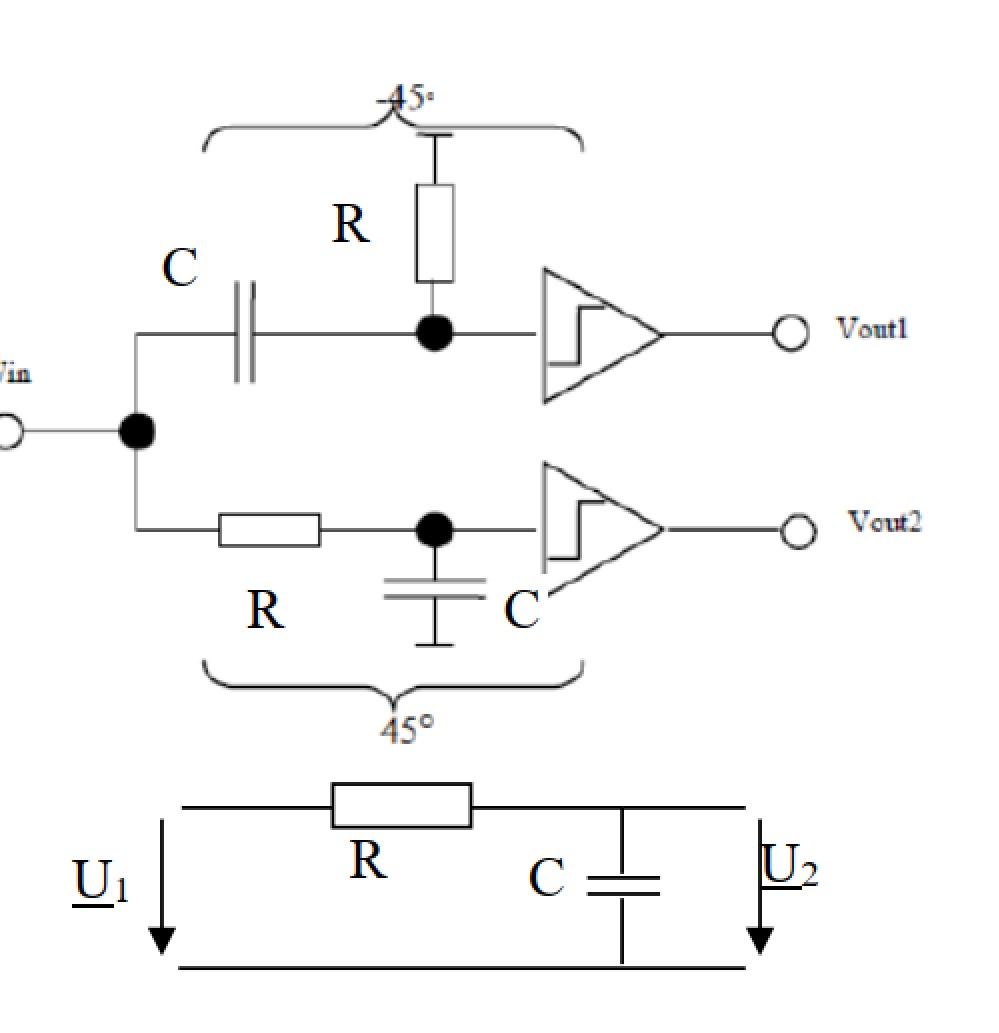
\includegraphics[width=8cm]{images/phase_shifter.jpg}
  \caption{phase shifter}
  \label{fig:phase_shifter}
\end{figure}
\paragraph{DC offset in zero-IF receivers/ self-mixing process}
Assume that the LO power of a zero-IF receiver is given by PLO=0dBm. All impedances are Zo=50
$\Omega$. The isolation between the mixer's LO port and the LNA's input port is 60dB (when connected
at the antenna). The amplification of the combination of LNA and Mixer is 30dB.

Calculate the resulting voltage at the mixer's output. Compare this voltage with the the rms value
of the voltage resulting from an RF signal of -80dBm at the antenna footpoint.\newline\newline
Note: The figure of 30dB isolation between LO and RF port is with connected antenna i.e. the
coupled LO power is divided by 2, one half travelling towards the antenna, the other half travelling
towards the LNA input port.\newline
DC power at mixer's output: (0-30-30+30) dBm = -30 dBm $Rightarrow$ 7mV @ 50$\Omega$
RF power at mixer's output: (-80+30) dBm = -50 dBm $Rightarrow$ 0.7mV rms @ 50$\Omega$\newline
the DC offset voltage is 10x higher as a reasonably strong RF input signal!
\paragraph{Even-order distortion in zero-IF receivers}
Show that zero-IF receivers are susceptible(anfällig) to even-order distortions.\newline\newline
Second order nonlinearity: $y=x^2$\newline
$$
\begin{aligned}
& x(t):=x_1(t)+x_2(t) \\
& x_1(t)=\cos \left(\omega_1 \cdot t\right) \quad x_2(t)=\cos \left(\omega_2 \cdot t\right) \\
& \Rightarrow y(t)=\left[\cos \left(\omega_1 \cdot t\right)+\cos \left(\omega_2 \cdot t\right)\right]^2=\cos ^2\left(\omega_1 \cdot t\right)+\cos ^2\left(\omega_2 \cdot t\right)+2 \cdot \cos \left(\omega_1 \cdot t\right) \cdot \cos \left(\omega_2 \cdot t\right)= \\
& \cos ^2\left(\omega_1 \cdot t\right)+\cos ^2\left(\omega_2 \cdot t\right)+\left\{\cos \left[\left(\omega_1+\omega_2\right) \cdot t\right]+\cos \left[\left(\omega_1-\omega_2\right) \cdot t\right]\right\}
\end{aligned}
$$
If $\omega_1 \approx \omega_2$ then the component $\left(\omega_1-\omega_2\right)$ is a signal near DC, which could interfere with the downconverted wanted signal.
\paragraph{Choice of Receiver Topology}\mbox{}\\
Give some examples how the choice of receiver topology could be influenced by circuit design, economical or other issues. 

\begin{itemize}
    \item Advances in semiconductor technology $\Rightarrow$ higher clock frequencies$\Rightarrow$ possibility to realize certain signal processing functions digitally, which wasn't possible before due to bandwidth limitations, e.g. filtering
    \item Advances of semiconductor technology for computing applications $\Rightarrow$ large volume production $\Rightarrow$ price drop $\Rightarrow$ possibility of application of technology in novel applications for wireless telecommunication systems
\end{itemize}





\paragraph{Superheterodyne Receiver}\mbox{}\\
Discuss the advantage/disadvantage of having the bandpass before and after the amplifier in a superhet receiver with respect to receiver performance:


When the amplifier is before the filter the total noise figure will be improved, but the large signal behaviour becomes worse. Therefore, when one wants high sensitivity the amplifier must be at the beginning, whereas when one wants good large signal behaviour the amplifier must come after the filter.
\paragraph{Superheterodyne Receiver}\mbox{}\\
A receiver has to be designed covering a receiving frequency range between 118...136 MHz.
Determine the lowest possible intermediate frequency in order to be able to remove any image
frequency by an RF filter in front of the mixer stage.
Determine the local oscillator's frequeny range for this case for the two possibilities $f_{RF}<f_{LO}$f and
$f_{RF}<F_{LO}$f. Considering the result of b), which problem arises if an IF near the minimum IF is used? What would be the minimum value of the IF to circumvent the problem in c)? Discuss advantages and disadvantages to select the LO frequency above or below the receiving frequency\newline\newline
\begin{enumerate}
    \item From \autoref{eq:image_frequency} we know that $f_{I M}=f_{R F} \pm 2 f_{I F}$. Furthermore, one can see from \autoref{fig:image_freq_1} that $f_{I F}$ must at least be $\frac{1}{2}$ of the bandwidth of the signal which is $f_{I F} > \frac{1}{2}\cdot (f_{RF_{max}}-f_{RF_{max}})=9MHz$.
    \item According to \autoref{eq:mixer_output} $f_{I F}=\left|f_{R F} \pm f_{L O}\right|$ furthermore, the sign is minus for the case where $f_{L F}<f_{R F}$ due to that and the fact that $f_{R F}-f_{L F}=9MHz$ must always be true $f_{L F}$ has a range from 109-127MHz. For the case where $f_{L F}>f_{R F}$ the sign is opposite and therefore in the range 127MHz-145MHz.
    \item 
    \begin{itemize}
        \item The leakage from LO to RF port (typically in the order of -30dB) may be partially reflected at the antenna port and then self-mixed with the LO signal. This results in a DC component in the downconverted signal. As long as the receiver topology is an IF topology, this DC component can be removed by high pass or band pass filtering. However, if the receiver topology is a zero-IF topology, then it is difficult if not impossible to remove this offset.
        \item Moreover, the LO leakage signal passes the RF input filter backwards and may be reradiated by the receiving antenna. To avoid this re-radiation, the LO frequency range must be placed out of the receiving frequency range $\Rightarrow$ possibility to reject backwards path by the RF bandpass
    \end{itemize}
    \item To avoid the second problem in c):
    $$
    \begin{aligned}
    \text { Aussuming } f_{\mathrm{LO}}<f_{\mathrm{RF}} & \Rightarrow f_{\mathrm{LO}, \max }<f_{\mathrm{RF}, \min } \\
    & f_{\mathrm{RF}, \max }-f_{\mathrm{IF}}<f_{\mathrm{RF}, \min } \\
    & f_{\mathrm{IF}}>f_{\mathrm{RF}, \max }-f_{\mathrm{RF}, \min }=18 \mathrm{MHz}
    \end{aligned}
    $$
    \item $\mathrm{f}_{\mathrm{LO}}<\mathrm{f}_{\mathrm{RF}}$\newline
    Advantages:
    \begin{itemize}
        \item lower frequency range
        \item spectrum at IF is not inverted
    \end{itemize}
    \textbf{Disadvantages:}
    \begin{itemize}
        \item bigger relative bandwidth
    \end{itemize}
    $f_{L O}>f_{R F}$ vice versa
\end{enumerate}





\paragraph{Dual-IF topology with image-signal rejection}\mbox{}\\
A given dual-IF topology (see above figure) has the following specifications:\newline
$f_{R F}$ = 87.5MHz...108 MHz\newline
Bandwidth of the received signal: B=180kHz\newline
First IF at $f_{IF_1}$=10.7 MHz\newline
Second IF at $f_{IF_2}$=455 kHz\newline
$f_{LO_1}<f_{RF}$\newline
Determine all spurious signals which could occur due to the selection of this set of intermediate
frequencies if the RF input frequency is given by $f_{R F}$ = 90.7 MHz.
Why is Filter 2 in \autoref{fig:double_superheterodyne_receiver} needed?
What is the maximum bandwidth of Filter 2 in \autoref{fig:double_superheterodyne_receiver} to fulfil its function (see b))?

\begin{enumerate}
    \item 
    \begin{itemize}
        \item $f_{\mathrm{LO} 1}=\mathrm{f}_{\mathrm{RF}}-\mathrm{f}_{\mathrm{IF} 1}=90.7 \mathrm{MHz}-10.7 \mathrm{MHz}=80 \mathrm{MHz}$
        \item 2 possible cases for $f_{\mathrm{LO2}}$ :
        \begin{itemize}
            \item $f_{\mathrm{LO2}}<f_{\mathrm{IF} 1}:  f_{\mathrm{LO2}}=\mathrm{f}_{\mathrm{IF} 1}-\mathrm{f}_{\mathrm{IF} 2}=10.7 \mathrm{MHz}-0.455 \mathrm{MHz}=10.245 \mathrm{MHz}$
            \item $f_{\mathrm{LO2}}>\mathrm{f}_{\mathrm{IF} 1}:  \mathrm{f}_{\mathrm{LO2}}=\mathrm{f}_{\mathrm{IF} 1}+\mathrm{f}_{\mathrm{IF} 2}=10.7 \mathrm{MHz}+0.455 \mathrm{MHz}=11.155 \mathrm{MHz}$
        \end{itemize}
        \item Other mixing products
        $$\begin{aligned} \mathrm{f}_{\mathrm{IF} 1}^{\prime} & =\mathrm{f}_{\mathrm{RF}}+\mathrm{f}_{\mathrm{LO} 1}=90.7 \mathrm{MHz}+80 \mathrm{MHz}=170.7 \mathrm{MHz} \\ & \Rightarrow \text { Has to be rejected by } \mathrm{BPF}_{3} ! \\ \mathrm{f}_{\mathrm{IF2} 2}^{\prime} & =\mathrm{f}_{\mathrm{IF} 1}+\mathrm{f}_{\mathrm{LO2}}=10.7 \mathrm{MHz}+10.245 \mathrm{MHz}=20.945 \mathrm{MHz}\left(\text { if } \mathrm{f}_{\mathrm{LO2}}<\mathrm{f}_{\mathrm{IF} 1}\right) \\ \mathrm{f}_{\mathrm{IF} 2}^{\prime} & =\mathrm{f}_{\mathrm{IF} 1}+\mathrm{f}_{\mathrm{LO2}}=10.7 \mathrm{MHz}+11.155 \mathrm{MHz}=21.855 \mathrm{MHz}\left(\text { if } \mathrm{f}_{\mathrm{LO2}}>\mathrm{f}_{\mathrm{IF} 1}\right)\end{aligned}$$
    \end{itemize}
    \item Need of Filter 2
    \begin{itemize}
        \item To reject other than the wanted mixing product of mixer 1
        \item To work as an image-reject filter for the second mixer stage
    \end{itemize}
    \item The situation can be seen in \autoref{fig:image_ex_1} and \autoref{fig:image_ex_2}. Filter 2 in \autoref{fig:double_superheterodyne_receiver} must therefore at least block the image frequencies, when $f_{LO_{2,2}}$ is chosen it must block at least all frequencies that are higher than 9.79MHz+0.09MHz=9.88MHz
    
\end{enumerate}
\begin{figure}[ht]
  \centering
  \resizebox{1\textwidth}{!}{\subimport{images/}{spectrum_1.tex}}
  \caption{Image frequencies with bandpass}
  \label{fig:image_ex_1}
\end{figure}

\begin{figure}[ht]
  \centering
  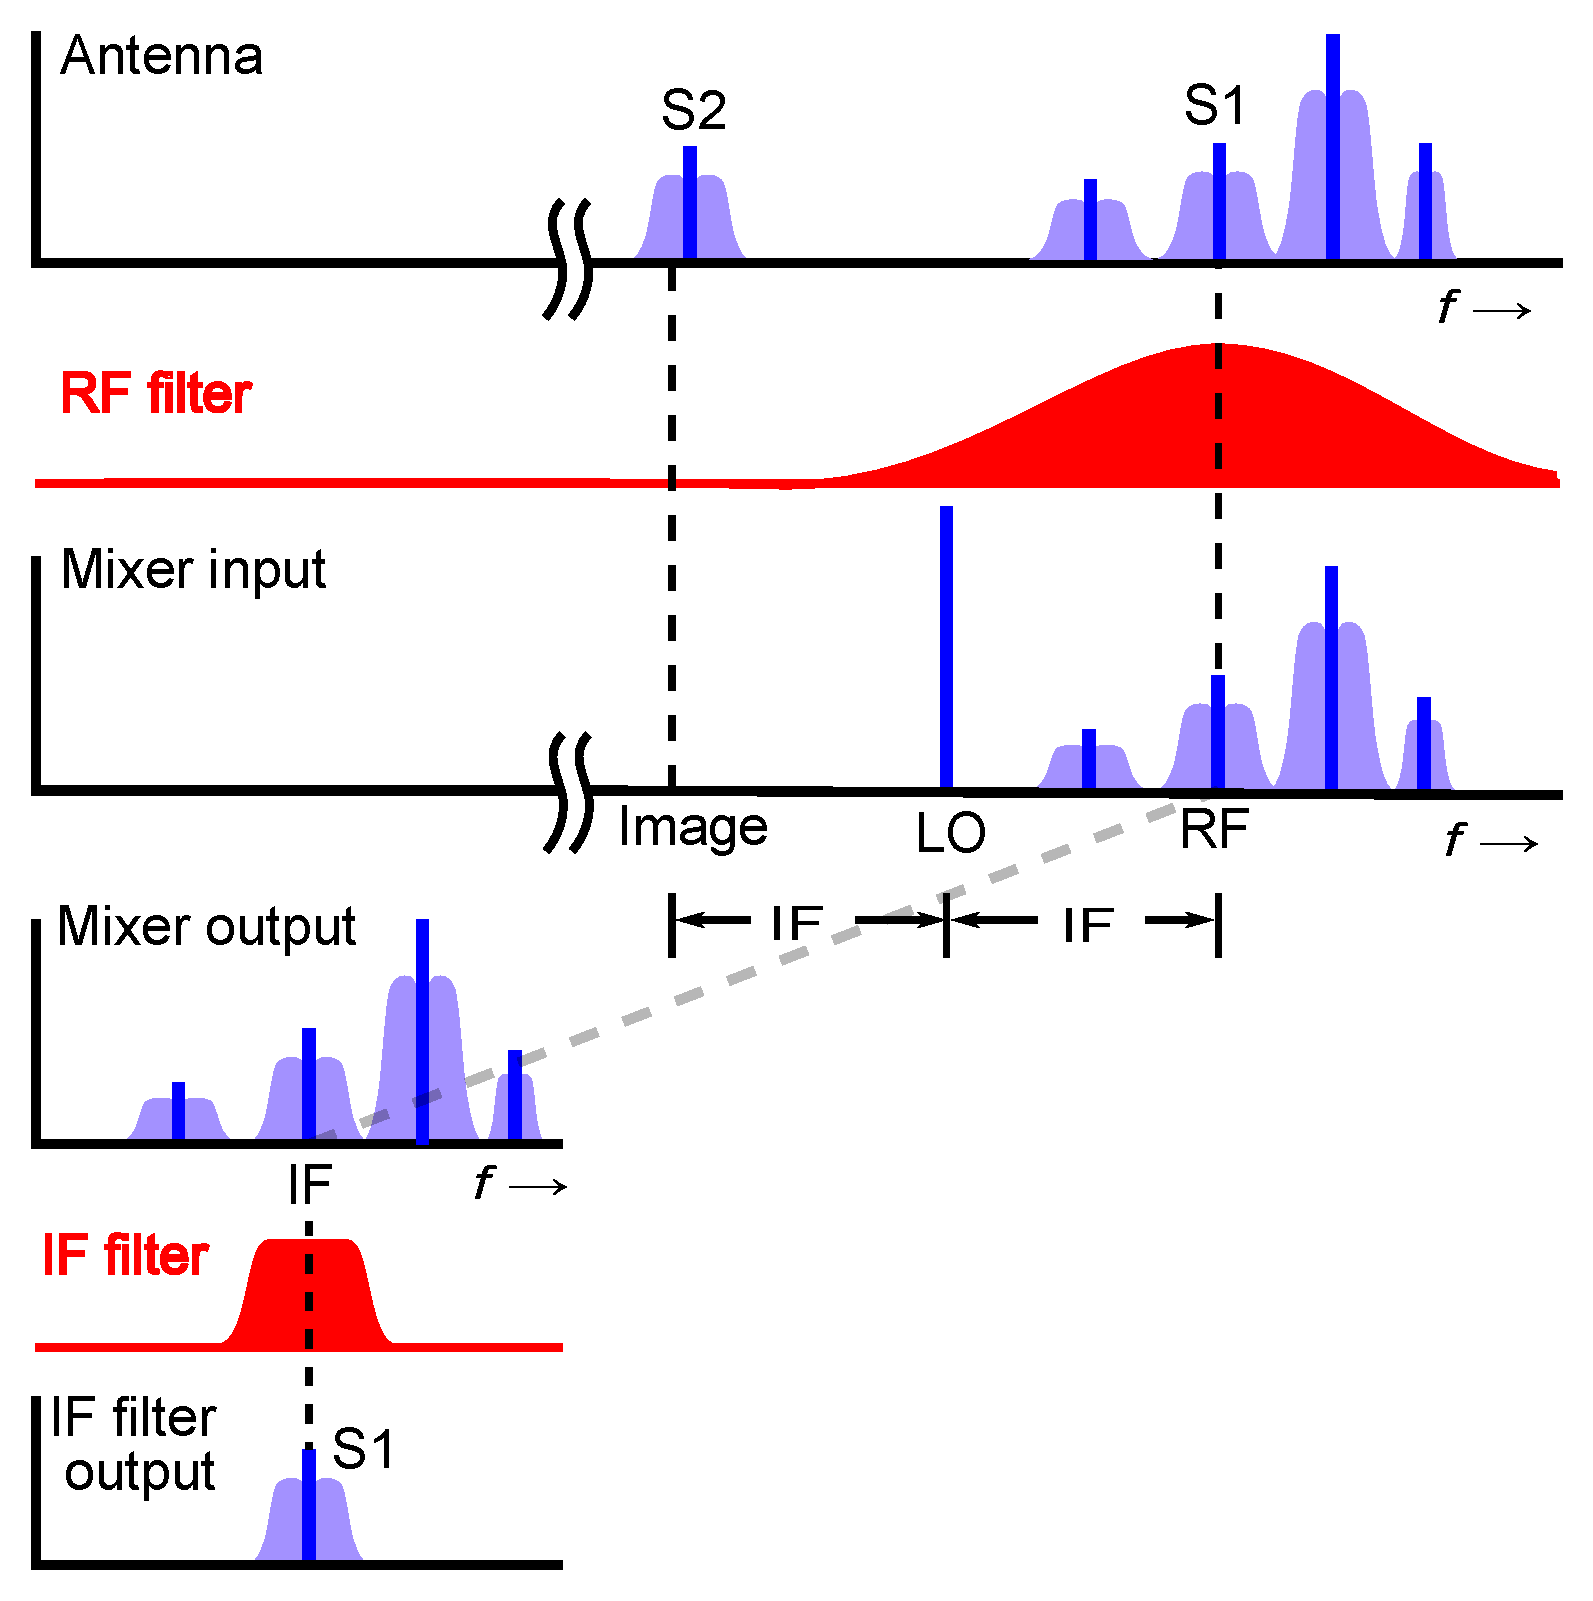
\includegraphics[width=8cm]{images/Superheterodyne2.pdf}
  \caption{superheterodyne radio principle}
  \label{fig:typical_superheterodyne_receiver_principle}
\end{figure}
\begin{figure}[ht]
  \centering
  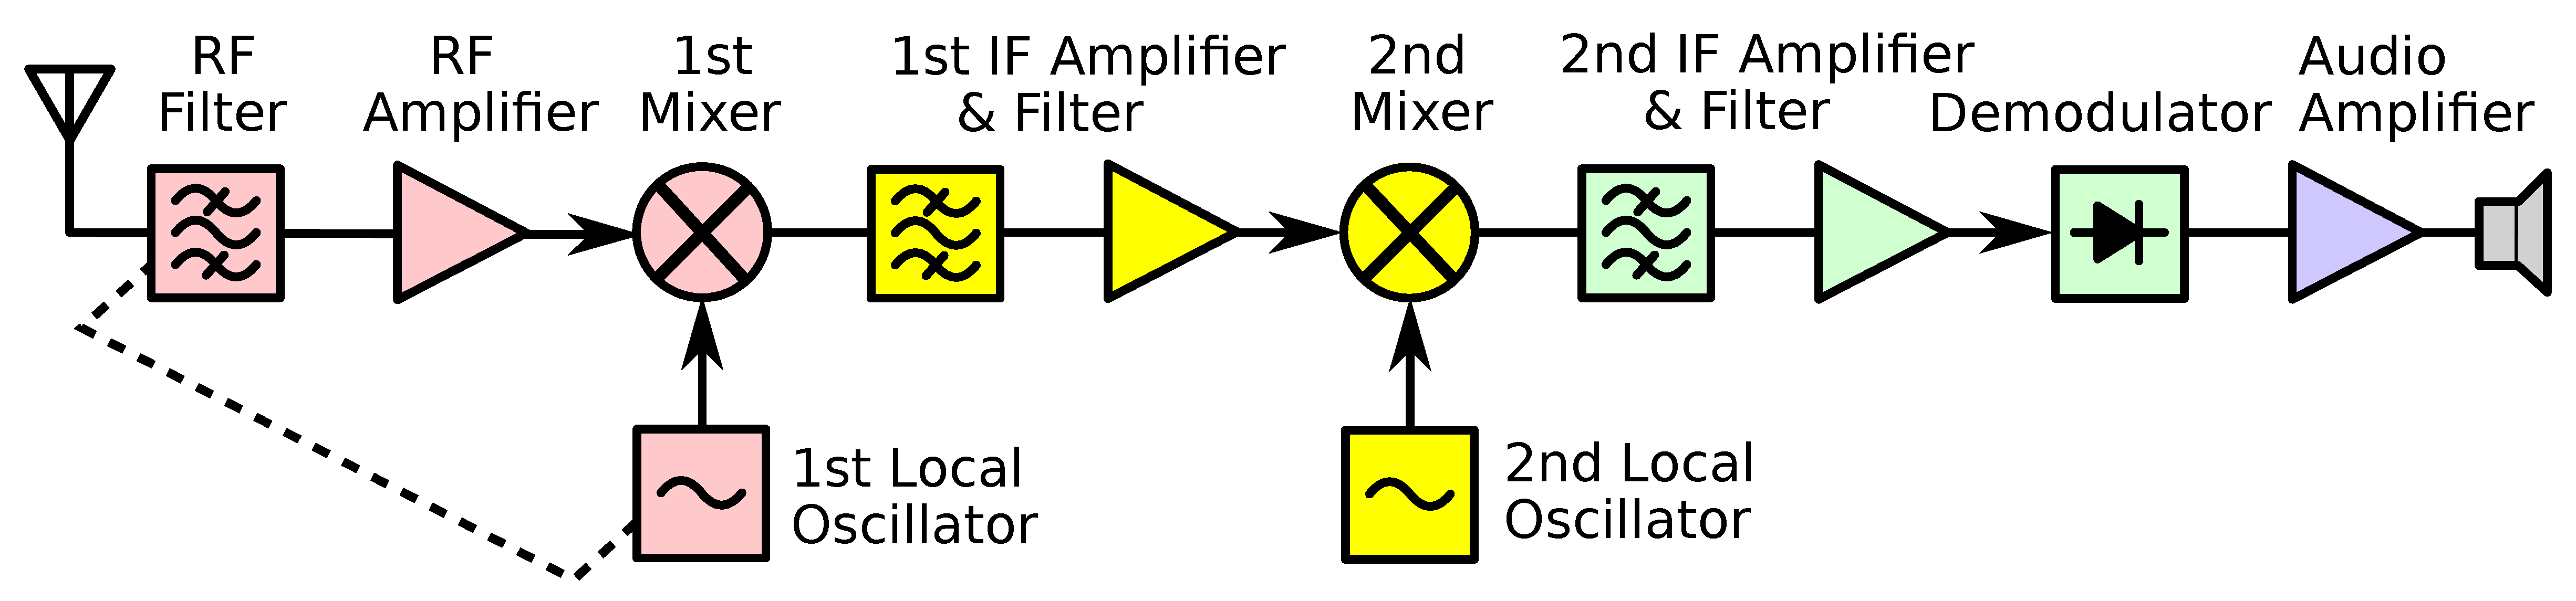
\includegraphics[width=8cm]{images/Superheterodyne3.pdf}
  \caption{Double conversion superheterodyne receiver block diagram}
  \label{fig:double_superheterodyne_receiver}
\end{figure}



\begin{figure}[ht]
  \centering
  \resizebox{1\textwidth}{!}{\subimport{images/}{spectrum_2.tex}}
  \caption{Image frequencies with bandpass}
  \label{fig:image_ex_2}
\end{figure}
\begin{figure}[ht]
  \centering
  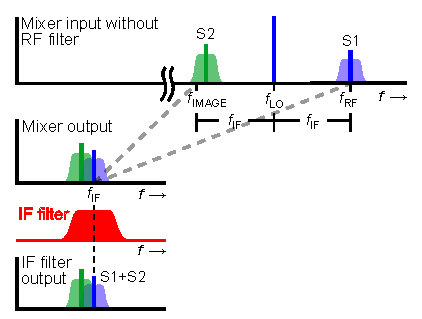
\includegraphics[width=8cm]{images/Superheterodyne4.pdf}
  \caption{illustrating for the problem of image response}
  \label{fig:image_response}
\end{figure}